\documentclass[journal]{IEEEtran}
\usepackage[spanish]{babel}
\usepackage[utf8]{inputenc}
\usepackage{amsmath, amsthm, amsfonts}
\usepackage{graphicx}
\usepackage{cite}
\usepackage{listings}
\usepackage{tabularx}
\usepackage{multirow}                                  
\usepackage{colortbl}
\renewcommand{\refname}{Referencias}
\usepackage{subfig}
\usepackage{booktabs}
\usepackage{cite}
\usepackage{float}
\usepackage{captdef}
\usepackage{textcomp}

\usepackage{fancyhdr}

\renewcommand{\citedash}{ -- } 

\renewcommand{\tablename}{\small{\textsc{Tabla}}}

\begin{document}


\title{Memoria de cálculo de diseño sistema fotovoltaico On grid sin inyección a red}
%\author { Bryan David Rosas Rojas - 97071908228\\  bdrosasr @unal.edu.co  }
\maketitle

\IEEEpeerreviewmaketitle

%\begin{abstract}
%\end{abstract}

\subsection*{Objetivo}
1. Determinar un diseño que sea capaz de alimentar las cargas del tercer piso del colegio xx ubicado en la ciudad de Yopal, Casanare sin inyectar los excedentes a la red almacenándolos en un banco de baterías\\

Asumiendo que las luminarias tengan un funcionamiento de 10h por día, y que la carga de las tomas sería de 720W por 3h durante el día, se tiene un consumo aproximado de 5kWh/día. Por otro lado, tenemos que la radiación solar mínima es de 4186HSP y máxima de 5760HSP ---según las tablas multianuales del ideam---, de esta forma se genera mínimo 6,5kWh y máximo 8,9kWh durante el día, por está razón se decide almacenar por lo menos 3kWh de está energía por medio del banco de baterías.


%\section*{I.se realizará con el o resitectrodo INTRODUCCImesticosÓN}


%\section*{II. MARCO TEÓRICO}
\section*{CÁLCULOS}
Para determinar la dimensión del banco de baterías, se tiene como parámetro, el nivel de tensión del inversor que soporta, la cantidad de energía que se desea almacenar, una capacidad de descarga igual al 70\% (son baterías de gel), un día de autonomía y 10\% de pérdidas, teniendo en cuenta esto, se tiene que:
\subsection*{BATERÍAS}
Se tienen las siguientes ecuaciones:

\begin{equation}
    Capacidad_{descarga}= \dfrac{energía_{ponderada} *días_{ autonomía}}{profundidad_{descarga}}
\end{equation}

\begin{equation}
Capacidad_{bateria}= \dfrac{Capacidad_{descarga}}{Tensión}
\end{equation}

Reemplazando:
\begin{equation}
    Capacidad_{descarga}= \dfrac{3kWh*1}{0.7}= 4.285kWh*día
\end{equation}

\begin{equation}
Capacidad_{bateria}= \dfrac{4.285}{24} = 180Ah
\end{equation}

Ahora, como necesitamos aproximadamente 180Ah, se elige un banco de baterías compuesto por 4 unidades, cada una con una capacidad de 100Ah y un nivel de tensión de 12V, se realiza una conexión mixta, dos arreglaos de baterías en paralelo conectadas en serie, como indica la siguiente figura: \\

\begin{figure}[H]
    \centering
    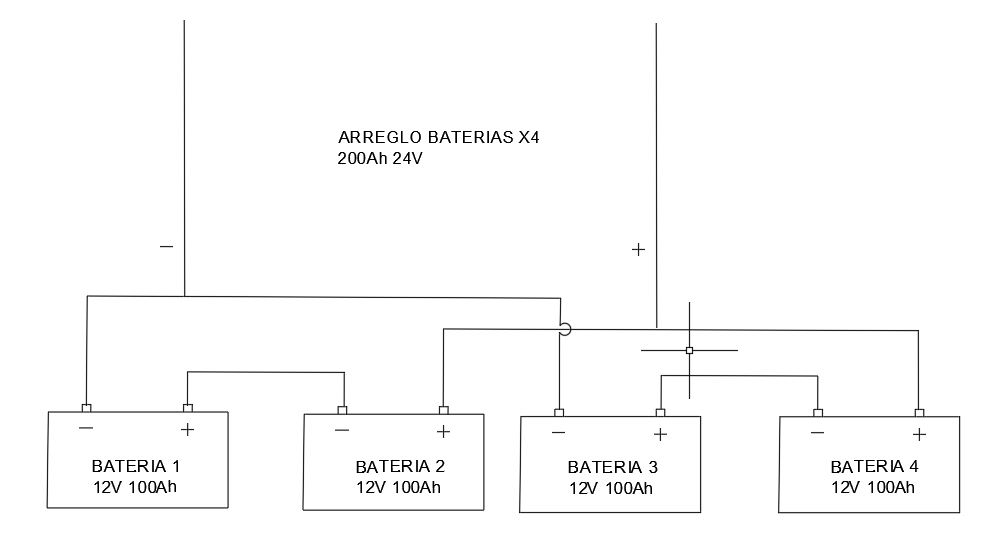
\includegraphics[scale=0.4]{Array_bat.JPG}
    \caption{Configuración conexión baterias}
    \label{curva}
\end{figure}





\subsection*{REGULADOR}
El regulador es un mppt que viene integrado con el inversor, su voltaje de operación se encuentra entre 30 a 115VDC.

\subsection*{INVERSOR CARGADOR}
El inversor cargador es un POWEST de 3kVA monofásico con un f.p de 0.8, es decir que entrega una potencia activa de 2400W, se eligió este por la capacidad de corriente y tensión que admite de las baterías, por el nivel de tensión que aguanta su mppt de la entrada del arreglo fotovoltaico, trabaja con un nivel de frecuencia de 60Hz y entrega una corriente nominal de 25A a 120V AC. Además, permite la conexión de baterías tipo gel y se puede monitorear desde su pantalla LCD o desde el software que suministra para computador.\\

El diagrama del esquema general es el siguiente:\\

\begin{figure}[H]
    \centering
    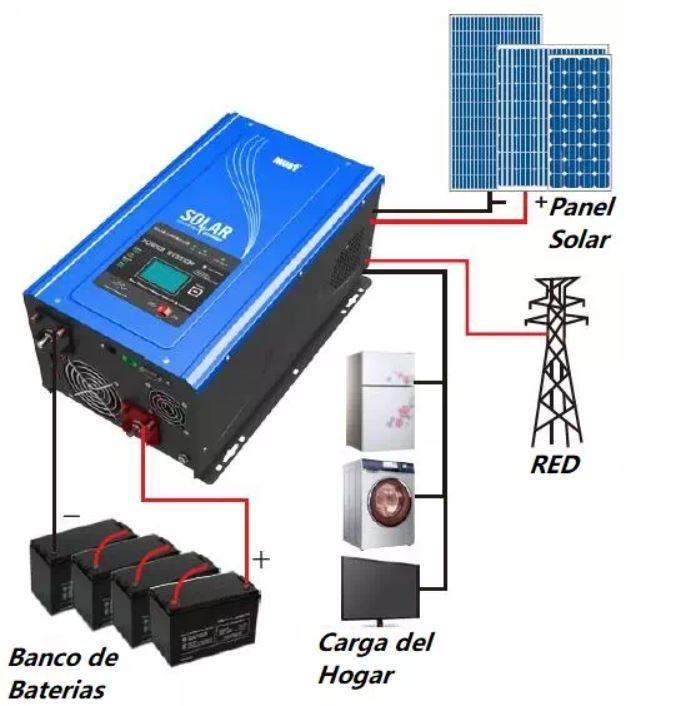
\includegraphics[scale=0.4]{esq_inv.JPG}
    \caption{Esquema general planta generación solar con baterías}
    \label{curva}
\end{figure}


\subsection*{PANELES SOLARES}
Debemos tener en cuenta el voltaje máximo que puede soportar el Regulador, ya que si la tensión de circuito abierto es mayor podría quemarse. También tener en cuenta la corriente máxima que soporta y tener en cuenta la tensión de entrada del inversor y la caída de tensión en el regulador para diseñar el sistema fotovoltaico.  Teniendo en cuenta lo anterior, se eligió: \\
Un arreglo fotovoltaico compuesto por 4 paneles conectados como se ve en la siguiente figura:\\


\begin{figure}[H]
    \centering
    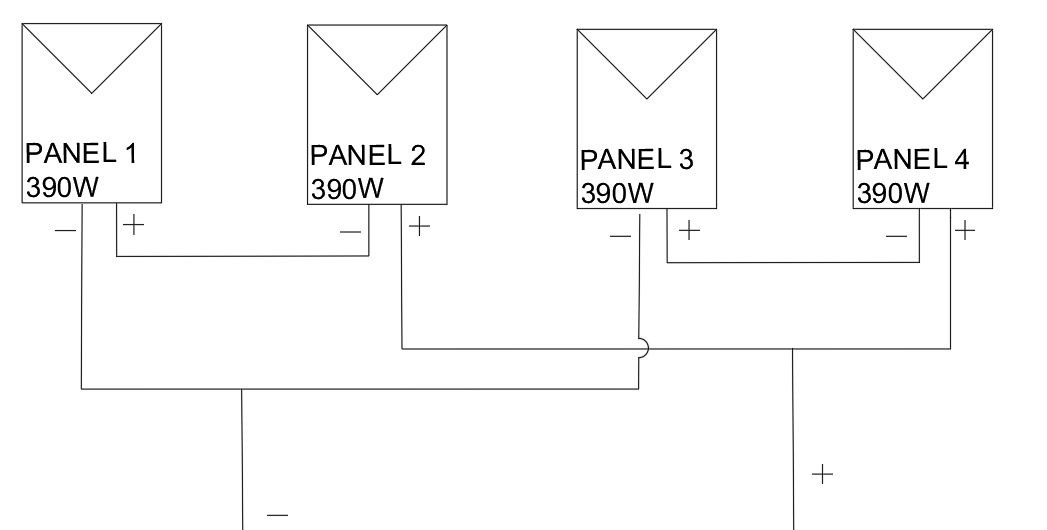
\includegraphics[scale=0.4]{arrayPV.JPG}
    \caption{Configuración conexión paneles solares}
    \label{curva}
\end{figure}

Además, se tiene que generan al día la siguiente cantidad de energía:
\begin{equation*}
   Energía=Potencia_{pico}*{HSP}
\end{equation*}

\begin{equation*}
   Energía=390W*4*{4,186}
\end{equation*}
\begin{equation*}
   Energía=6,5 \dfrac{kWh}{día}
\end{equation*}
Se eligieron 4 paneles marca Jinko, modelo (Cheetah HC 72M JKM390M-72H). 
Con una potencia pico de 390W, Vmp=41,1V, Imp=9,49A, Voc=49,3V, Isc=10,12A, 19,38\% de eficiencia, con un tamaño de 2,008m*1,002m 
y un peso de 22,5kg. Su conexión es la siguiente:\\

\section*{CABLEADO}

\subsection*{SOLAR DC}

Para la conexión entre los paneles para formar el arreglo fotovoltaico en serie, se elige 4 extensiones de cable que ya viene con los MC4 de 1 metro y 12AWG cada uno. Y para realizar la conexión entre el paralelo de los dos paneles en serie, se elige un conector MC4 Y doble 2 en 1 de 12AWG, para conectar el cable solar al fusible MC4 se eligio un cable solar de longitud de 10m rojo y negro de 12AWG, con 2 conectores MC4, además con esta cantidad de cable ir desde el fusible hasta la protección y de la protección al inversor con cable 12AWG. 

\subsection*{BATERIAS DC}
Para la conexión serie entre baterías se elige un calibre 8AWG para que soporte hasta 100A ya que el inversor soporta hasta 132A. El cable es utilizado para conexiones entre las baterías, conexión a la protección DC y conexión con el inversor cargador. 

\subsection*{AC}

Se define que la configuración del inversor debe estar programada para que la batería se cargue solamente con la generación solar, no con la red, cuando no haya suficiente potencia para suplir la carga de los circuitos 13 y 14, el inversor funciona como un by pass y le da paso a la red para suplir la potencia de las cargas.\\
Por esta razón, el cable que proviene del tablero principal del edificio (aguas abajo de la red) a alimentar el inversor, será un 3x12AWG (1 fase, neutro y tierra). \\

A la salida del inversor para alimentar el tablero del tercer piso, donde se encuentran los circuitos 13 y 14. El cable será un 3x12AWG (1 fase, neutro y tierra) debido a que:\\
$$I=\dfrac{1500VA}{120V}*1.25=15,62A$$
Para la alimentación de los circuitos 13 y 14, previamente habían elegido un 3x12AWG. 
\section*{PROTECCIONES}

\subsection*{FUSIBLES}

Como tenemos una potencia pico de 1560Wp y un nivel de tensión de 98,6V, calculamos la corriente:\\
$$Corriente_pv=\dfrac{1560Wp}{98,6V}=15,82A$$
Por lo tanto, se elige un fusible de 20A MC4 IP68 para el lado positivo y el lado negativo. \\

Para las baterías es recomendable colocar un fusible en cada polo, y como se eligió un calibre de 8AWG, se selecciona un fusible de 100A con su respectivo porta fusibles.


\subsection*{PROTECCIONES DC}

Como la corriente que transitaría por el arreglo es de aproximadamente 18,96A, se elige una protección de 20A en DC para los paneles.\\



\subsection*{PROTECCIONES AC}

Se elige una protección de 20A para el circuito que viene del tablero principal a energizar el inversor. La protección de salida del inversor que alimenta el tablero del tercer piso es de 20A. 



\section*{TUBERÍA}

El cable solar que proviene de los paneles tiene la capacidad de resistencia a la interperie, por está razón no requiere tubería.\\
Para la tubería AC, desde el tablero del 3er piso se elige una tubería SCH80 de 1" que llegue hasta el gabinete de la sotea que contiene los equipos de la instalación fotovoltaica, si por alguna razón la tubería queda expuesta en la sotea, se elige una tubería EMT de 1" que vaya desde la caja de paso de uso externo hasta la entrada del gabinete de la planta solar. 

\section*{ESTRUCTURA}

Para la estructura de los paneles se eligieron 8 kit single fix-v para sujetar el riel de soporte de los modulos al techo que se encuentra en la institución, la conexión se hará de la siguiente manera: \\

\begin{figure}[H]
    \centering
    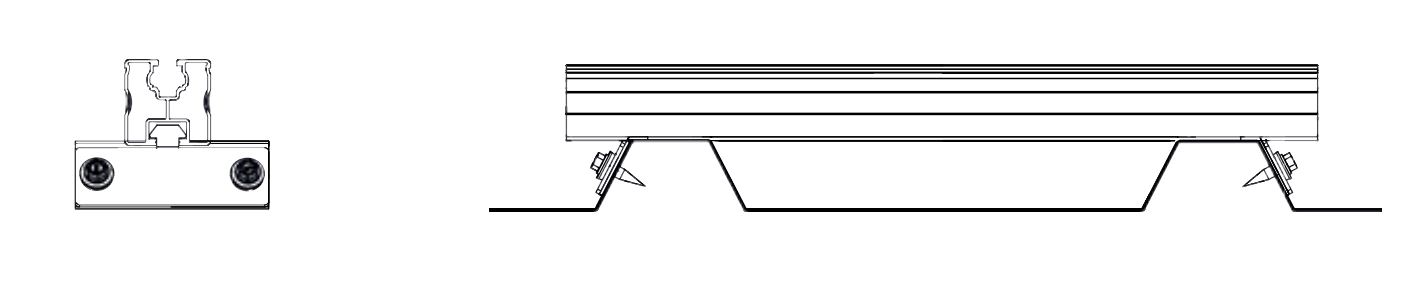
\includegraphics[scale=0.3]{anclaje_estrucJPG.JPG}
    \caption{Anclaje de los rieles de los paneles al techo}
    \label{curva}
\end{figure}



%\section*{V. ANÁLISIS DE RESULTADOS }

%\section*{V. CONCLUSIONES}
%1. Podría ser causa la nevera del aumento del recibo de pago de la electricidad, debido a la operación deficiente de su motor y teniendo en cuenta que el consumo en general de la casa permanece igual o menor en comparación con el promedio de consumo durante varios años.\\
%2. La importancia de saber el estado de funcionamiento y cuanta energía consume un electrodomestico, con el fin de bajar el consumo de energía eléctrica. 
%\section*{VI. BIBLIOGRAFÍA}







\end{document}
